\subsection {Inteligencia artificial}\label{subsec:intela}
\begin{wrapfigure}[3]{r}[0cm]{2.666cm}
	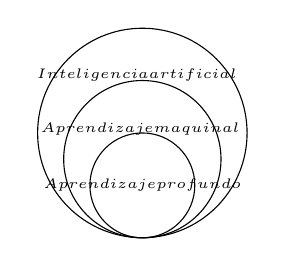
\begin{tikzpicture}
	\def\IA{(0,0) circle (1.33cm)}
	\def\AM{(270:.333cm) circle (.999cm)}
	\def\AP{(270:.666cm) circle (.666cm)}
	\draw \IA node[above]{\tiny$^{^{^{^{^{^{^{^{\overunderset{\text{ Inteligencia}}{\text{ artificial}}{}}}}}}}}}$};
	\draw \AM node[above]{\tiny$^{^{^{\overunderset{\text{Aprendizaje}}{\text{maquinal}}{}}}}$};
	\draw \AP node{\tiny$\overunderset{\text{Aprendizaje}}{\text{profundo}}{}$};
\end{tikzpicture}\caption[Inteligencia artificial]{\\Inteligencia\\artificial}\label{FIG:IA}
\end{wrapfigure}
\begin{displayquote}
el esfuerzo por automatizar tareas intelectuales normalmente realizadas por humanos(\citeauthor{cho18}, \citeyear{cho18})
\end{displayquote}
de este campo general se desprenden el \emph{aprendizaje maquinal} y el \emph{aprendizaje profundo}, figura (\ref{FIG:IA}).

Se pretende que la IA se acerque al funcionamiento de la mente humana, y se recurre a ella cuando se considera útil incorporar a un sistema de ordenadores un conocimiento o comportamiento ante los eventos que serían más propios de un ser humano.

\citeauthor{mich19} (\citeyear{mich19}) define aprendizaje maquinal como\begin{displayquote}
un programa de computadora aprende de experiencia $E$ con respecto a una tarea $T$ y una medición de rendimiento $P$, si su rendimiento en $T$, medido por $P$, mejora con $E$
\end{displayquote}
es decir, a diferencia del paradigma clásico de programación donde los humanos introducen datos y órdenes para procesarlos, un sistema de aprendizaje maquinal no se programada explícitamente, se introducen muchos ejemplos relevantes a una tarea (datos y respuestas esperadas) con los que es entrenado y si encuentra una estructura estadística en ellos, genera una regla para automatizar la tarea.

El \emph{procesamiento de lenguaje natural} (PLN), es el conjunto de métodos para hacer accesible el lenguaje humano a las computadoras(\citeauthor{eise19}, \citeyear{eise19}). Toma conocimientos de muchas tradiciones intelectuales, como lingüística y teoría formal del lenguaje, autómatas y otras áreas computación, inteligencia artificial, aprendizaje maquinal y profundo, estadística, teoría de la información, fonética y fonología, estas dos últimas áreas son de particular utilidad para procesamiento de voz. Existen dos posturas opuestas sobre lo que la tarea principal del PLN debe ser:
\begin{itemize}
	\item Entrenar sistemas de principio a fin para que transmuten texto sin procesar en cualquier estructura deseada.
	\item Transformar texto en una pila de estructuras lingüísticas de uso general que en teoría deben poder soportar cualquier aplicación.
\end{itemize}
En la actualidad no hay consenso y ambos tipos de sistemas se consideran viables, este proyecto se basará en el segundo paradigma. 

Por lo general el PLN divide sus funciones en módulos para facilitar la reutilización de algoritmos genéricos en diversas tareas y modelos, dos de los módulos básicos son \emph{búsqueda} y \emph{aprendizaje} con los que se puede resolver muchos problemas que tienen la forma matemática
\begin{equation}
\begin{matrix}
\hat{y}=argmax\Psi(x,y;0),\\
y\in Y(x)
\end{matrix}\label{EQ:NLP1}
\end{equation}
donde,
\begin{itemize}
	\item $x$ es la entrada, un elemento de un conjunto $X$.
	\item $y$ es el resultado, un elemento de un conjunto $Y$.
	\item $\Psi$ es una función de puntuación (también conocida como \emph{modelo}), que va desde el conjunto $X\times Y$ hasta los números reales.
	\item $\emptyset$ es el vector de parámetros para $\Psi$.
	\item $\hat{y}$ es el resultado previsto, que es elegido para maximizar la función de puntuación.
\end{itemize}
El módulo de búsqueda se encarga de computar el $argmax$ de la función $\Psi$, es decir, encuentra el resultado $\hat{y}$ con la mejor puntuación con respecto a la entrada $x$. El módulo de aprendizaje encuentra los parámetros $\theta$ por medio del procesamiento de grandes conjuntos de datos de ejemplos etiquetados ${\{(x^i,y^i)\}}_{i=1}^{N}$.

Un método lineal de clasificación de texto común es la \emph{bolsa de palabras}, comienza por asignar etiquetas $y\in Y$ donde $Y$ son todas las posibles etiquetas. Se utilizan vectores columna y la fórmula \ref{EQ:NLP1} y puede modelarse con diversas distribuciones (figura \ref{FIG:DISTS}).

Para muchas tareas, las características léxicas (palabras) pierden sentido en aislamiento, por lo que históricamente el PLN se ha enfocado en la clasificación lineal, recientemente algunas tareas pueden resolverse con clasificadores no lineales, es decir, por medio de redes neuronales (aprendizaje profundo).

El aprendizaje profundo sigue el paradigma del aprendizaje maquinal, sus entradas son datos y ejemplos de resultados esperados y se mide si el algoritmo está haciendo un buen trabajo mientras \emph{aprende}. A diferencia del aprendizaje maquinal, se hace énfasis en aprender en capas sucesivas de representaciones cada vez más sucesivas. ``Profundidad'' entonces refiere a cuántas capas contribuyen a un modelo.